\documentclass[a4paper,12pt]{report}
\usepackage[T2A]{fontenc}
\usepackage[utf8]{inputenc}
\usepackage[english,russian]{babel}
\usepackage{circuitikz}
\usepackage{wrapfig}
\usepackage{makecell}
\usepackage{tabularx}
\usepackage{graphicx}
\usepackage{gensymb}
\usepackage{cancel} %cancel symbol
\usepackage{amsmath,amsfonts,amssymb,amsthm,mathtools}
\usepackage{pgfplots}
\usepackage{pgfkeys}
%\usepackage[margin=3cm]{geometry}
\pgfplotsset{compat=1.12}
\usepackage{mathrsfs}

\usepackage[pagestyles]{titlesec}
\titleformat{\chapter}[display]{\normalfont\huge\bfseries\centering}   {\chaptertitlename\ \thechapter}{20pt}{\Huge}
\titlespacing{\chapter}{0pt}{-48pt}{1cm}

%tikz (draw)

\usepackage{tikz}
\usepackage{pstricks-add}
%tikz libraries

\usetikzlibrary{intersections}
\usetikzlibrary{arrows.meta}
\usetikzlibrary{calc,angles,positioning}
\usetikzlibrary{arrows}
\usepackage{float}

\parindent=0ex
\setlength{\parskip}{\baselineskip}%
\setlength{\parindent}{0pt}%

\graphicspath{ {C:/Users/George/Documents/MIPT_TEX/} }

\newcommand{\R}{{\mathbb R}}
\newcommand{\N}{{\mathbb N}}
\newcommand{\fancy}[1]{{\mathbb{#1}}}
\DeclareMathOperator{\sgn}{sgn}
\newtheorem{problem}{Задача}[]
\newenvironment{sol}{\paragraph{Решение}}{}
\renewcommand\thesection{\arabic{section}}
\newcommand{\uni}{\cup}
\newcommand{\inter}{\cap}

\begin{document}
	

\begin{titlepage}
	\begin{center}
		МОСКОВСКИЙ ФИЗИКО-ТЕХНИЧЕСКИЙ ИНСТИТУТ (НАЦИОНАЛЬНЫЙ ИССЛЕДОВАТЕЛЬСКИЙ УНИВЕРСИТЕТ) \\
		
		
		\hfill \break
		Факультет обшей и прикладной физики\\
		\vspace{2.5cm}
		\large{\textbf{Отчёт по лабораторной работе 1.2.5 <<Исследование прецессии уравновешенного гороскопа>>}}\\
		\hfill \break
		\\
	\end{center}
	
	\begin{flushright}
		Выполнил:\\
		Студент гр. Б02-304\\
		Головинов. Г.А.
	\end{flushright}
	
	\vspace{7cm}
	
	\begin{center}
		
\includegraphics[width=0.15\linewidth]{uni}
	\end{center}
	

	

	\vfill
	
	\begin{center} Долгопрудный, 2023 \end{center}
	
	\thispagestyle{empty}
	
\end{titlepage}


	\newpage
	\pagenumbering{arabic}
    
    \section*{Аннотация}
        \paragraph*{Цель работы:} измерить коэффициент теплопроводности воздуха при атмосферном давлении в зависимости от температуры.
        \paragraph*{В работе используются:} цилиндрическая колба с натянутой по оси нитью, термостат, вольтметр и амперметр, источник постоянного напряжения, магазин сопротивлений.

    \section*{Основные теоретические сведения}
    Теплопроводность -- процесс передачи тепловой энергии от нагретых частей системы к холодным за счет хаотического движения частиц среды. В газах теплопроводность осуществляется за счет непосредственной передачи кинетической энергии от быстрых молекул к медленным. Перенос тепла описывается законом Фурье.
    \paragraph*{Закон Фурье}
    Этот закон утверждает, что плотность потока энергии $\vec{q}$ (количество теплоты, переносимое через единичную площадку за единицу времени) пропорциональна градиенту температуры $\nabla T$:
    \begin{equation}
        \label{fourier}
        \vec{q}=-\varkappa \nabla T
    \end{equation}
    где $\varkappa$ -- коэффициент теплопроводности. [$\varkappa$]=$\frac{\text{Вт}}{\text{м}\cdot\text{К}}$

    Молекулярно-кинетическая теория дает оценку коэффициента теплопроводности газов:
    \begin{equation}
        \label{varkappa approx}
        \varkappa \sim \lambda \vec{v} \cdot n C_V
    \end{equation}
    здесь $\lambda$ -- длина свободного пробега молекул газа, $\vec{v}=\sqrt{\frac{8kT}{\pi m}}$ -- средняя скорость теплового движения, $n$ -- концентрация молекул, $C_V=\frac{i}{2}k$ -- теплоемкость при постоянном объеме в расчете на одну молекулу

    Формула \eqref{varkappa approx} дает лишь оценку по порядку величины, а также правильную функциональную зависимость. Коэффициент перед этой формулой зависит от закона взаимодействия молекул и не может быть вычислено методами общей физики. Также не подлежит прямому измерению длина свободного пробега.

    Ее можно оценить как $\lambda=1/n\sigma$, где $\sigma$ -- эффективное сечение столкновения молекул друг с другом -- величина, характеризующая вероятность существенного отклонения налетающей частицы при взаимодействии с некоторым рассеивающим центром. В общем случае определяется как отношение плотности потока рассеянных частиц к плотности потока падающих, имеет размерность площади.

    В простейшей модели $\sigma=const$, а коэффициент теплопроводности пропорционален корню абсолютной температуры: $\varkappa\sim\vec{v}/\sigma\sim\sqrt{T}$. На практике сечение $\sigma$ зависит от температуры и его следует считать медленно убывающей функцией.

    Рассмотрим теплопроводность в цилиндрической геометрии:
    \begin{wrapfigure}{R}{0.3\textwidth}
        \vspace{-5mm}
        \centering
        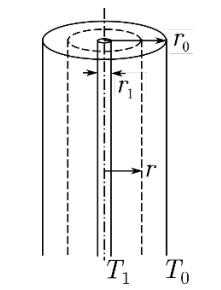
\includegraphics[width=0.7\linewidth]{img/geometry}
        \caption{Геометрия установки}
    \end{wrapfigure}

    Пусть тонкая нить радиусом $r_1$ и длиной $L$ помещена на оси цилиндра радиуса $r_0$. Температура стенок $T_0$ поддерживается постоянной. Пусть в нити выделяется некоторая тепловая мощность $Q$ [Вт]. Если цилиндр длинный ($L\gg r_0$), то можно пренебречь теплоотводом через его торцы. Тогда все параметры газа можно считать зависящими только от расстояния $r$ до оси цилиндра, а поток $\vec{q}$ -- направленным строго радиально (от оси).

    Вместо уравнения \eqref{fourier} имеем теперь:
    \begin{equation}
        \label{q new}
        q=-\varkappa\frac{dT}{dr}
    \end{equation}
    В стационарном состоянии полный поток тепла через цилиндрическую поверхность радиуса $r$ и площадью $S=2\pi rL$ должен быть одинаков и равен $Q=qS$:
    \begin{equation}
        \label{Q}
        Q=-2\pi r L\cdot \varkappa \frac{dT}{dr}=const
    \end{equation}
    Считая перепад температуры сильно меньшим чем само значение температуры ($\Delta \ll T_0$) можно пренебречь изменением теплопроводности $\varkappa$ от радиуса. Тогда можно проинтегрировать по радиусу и температуре:
    \begin{equation*}
        Q\int_{r_1}^{r_0}\frac{dr}{r}=-2\pi L\cdot \varkappa  \int_{T_1}^{T_0}dT 
    \end{equation*}
    \begin{equation*}
        Q\ln(r_0/r_1)=2\pi L \cdot \varkappa \Delta T, \quad \Delta T=T_1-T_0
    \end{equation*}
    \begin{equation}
        \label{Qfinal}
        Q=\frac{2\pi L\varkappa\Delta T}{\ln (r_0/r_1)}
    \end{equation}

    \paragraph*{Оценка времени установления равновесия} Когда в процессе работы мы меняем (желаемую) температуру на термостате требуется некоторое время, чтобы жидкость достигла этой температуры, затем некоторое время, чтобы жидкость достигла стенок цилиндра, затем некоторое время, чтобы воздух в цилиндре тоже прогрелся до новой температуры. Оценим время установления нового состояния в системе (без учета нагрева термостата).

    Рассмотрим плоский слой толщиной $a$ и сечением $S$, заполненный газом при постоянном давлении. Пусть температура одной из граней выросла на некоторую $\Delta T$. Это вызовет поток тепла в сторону более холодной грани, величину которого можно оценить по закону Фурье: $q\sim \varkappa \Delta T/a$. Для того чтобы весь слой прогрелся на $\Delta T$ в него должно поступить тепло $nSa\cdot C_p\Delta T$, где $C_p$ -- теплоемкость при постоянном давлении в расчете на одну молекулу.

    С другой стороны, поступившее за это время $\tau$ тепло можно вычислить как $qS\tau=\varkappa\frac{\Delta T}{a}S\tau$. Приравнивая находим:
    \begin{equation*}
        nSaC_p\Delta T=\varkappa\frac{\Delta T}{a}S\tau
    \end{equation*}
    тогда
    \begin{equation}
        \label{tau}
        \tau\sim\frac{C_pa^2n}{\varkappa}
    \end{equation}
    Коэффициент $\chi=\frac{\varkappa}{C_pn}$ называется температуропроводностью среды. Для воздуха при нормальных условиях $\chi\sim 0.2cm^2/s$, что при размере $a\sim 1cm$ имеет характерное время $\tau\sim 5s$

    Таким образом, состояние в установке может устанавливаться в течение нескольких десятков секунд, поэтому, учитывая также прогрев трубок, стоит ждать несколько минут после достижения термостатом желаемой температуры.

    \paragraph*{Пределы применимости теории} Закон Фурье может нарушаться, когда масштабы установки соизмеримы с длиной свободного пробега молекул. Это может привести к эффекту, известному как <<температурный скачок>>, явление, когда температура нити может отличаться от температуры окружающего газа. В данной работе этим можно пренебречь, так как при нормальных условиях $\lambda\sim 10^{-5}cm$, что сильно меньше размеров системы, и даже размеров нити.

    Также возможны другие механизмы теплопередачи: конвекция и излучение. Конвекция возникает в поле тяжести только при больших вертикальных градиентах температуры, поэтому установка расположена вертикально. Мощность излучения можно оценить по закону\newline Стефана-Больцмана:
    \begin{equation}
        \label{stef-bolz}
        Q_{rad}=\epsilon S \sigma_S(T_1^4-T_0^4)\approx 4\epsilon S\sigma_ST_0^3\Delta T
    \end{equation}
    где $S$ -- площадь поверхности нити, $\sigma_S=5.67\cdot 10^{-8}W/(m^2K^4)$ -- постоянная Стефана-Больцмана, $\epsilon$ -- безразмерный <<коэффициент черноты>>, зависящий от качества и материала излучающей поверхности. Для металлов с полированной поверхностью можно принять $\epsilon\sim 0.1-0.2$. По формуле \eqref{stef-bolz} находим мощность излучения:
    \begin{equation*}
        Q_{max} \approx 1.5mW
    \end{equation*}

    \subsection*{Экспериментальная установка}
    \begin{wrapfigure}{R}{0.5\textwidth}
        \vspace{0mm}
        \centering
        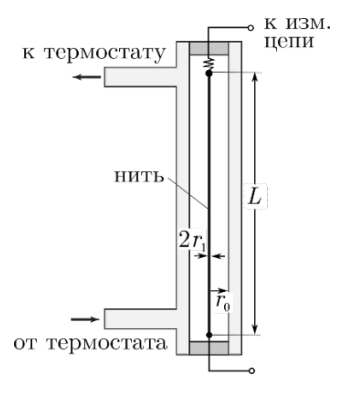
\includegraphics[width=0.7\linewidth]{img/ustanovka}
    \end{wrapfigure}

    Установка представляет собой цилиндрическую трубку длиной $L=40cm$, диаметром $2r_0=1cm$, диаметр нити $2r_1=50\mu m$. Трубка заполнена воздухом, через небольшое отверстие воздух внутри системы может сообщаться с атмосферой. Стенки трубки помещены в кожух, через который пропускается вода из термостата, так что температура стенок $T_0$ поддерживается постоянной. Трубка расположена вертикально для предотвращения влияния конвекции, как было обговорено ранее.

    Нить служит источником тепла:
    \begin{equation}
        \label{q wire}
        Q=UI
    \end{equation}
    где Q -- мощность нагрева нити, U -- напряжение на нити, I -- сила тока.
    
    Также нить является способом измерения температуры.  Сопротивление нити можно найти по закону Ома:
    \begin{equation}
        \label{ohm}
        R=\frac{U}{I}
    \end{equation}  
    
    Электрические приборы и нить подключены согласно следующей схеме:

    \begin{figure}[H]
    \centering
    \begin{circuitikz}[>=latex', european, scale=1.3]
    \tikzstyle{block} = [draw, rectangle, minimum height=1cm, minimum width=2cm]
    \draw (2.0,-0.0) to[R,l=$R$] (4.0,-0.0);
    \draw (0.0,-0.0) to[battery1,l=$\varepsilon$, invert] (2.0,-0.0);
    \draw (4.0,-0.0) to[R,l=$R_\text{н}$] (4.0,-3.5);
    \draw (4.0,-0.0) to[short] (5.5,-0.0);
    \draw (5.5,-0.0) to[rmeter, t=$U$] (5.5,-3.5);
    \draw (5.5,-3.5) to[short] (0.0,-3.5);
    \draw (0.0,-3.5) to[rmeter, t=$I$] (0.0,-0.0);
    \end{circuitikz}
    \caption{Схема цепи}
    \end{figure}

    Предполагая, что все компоненты цепи идеальны, измерив напряжение $U$ и силу тока $I$ можно найти мощность, выделяемую на нити и ее сопротивление. По этим данным мы будем строить зависимость $R(Q)$ -- нагрузочная кривая.

    Уменьшая сопротивление магазина мы увеличиваем значение силы тока в цепи. Есть некоторое значение силы тока $I_{max}$, выше которой теплопроводности воздуха перестанет хватать, чтобы отводить тепло, выделяющееся на нити. Если это значение превысить, нить может перегореть.

    Найдем максимальную мощность отвода воздуха по формуле \eqref{Qfinal}, затем используя формулу $Q_{w}=I^2 R$, считая $R\approx 20 \Omega$ получим, что $I_{max}\approx 137 mA$, если максимальная разница температур $\Delta T\approx 20 K$

    Зависимость $R(T)$ -- сопротивления от температуры при температурах около комнатной (0-100$C^\circ$) можно с достаточно большой точностью считать линейной зависимостью:
    \begin{equation*}
        R(T)\approx R_0(1+\alpha(T-T_0))
    \end{equation*}
    гда $\alpha$ -- коэффициент пропорциональности, $R_0$ -- сопротивление при температуре $T_0$.
    Мы в ходе работы также проверим ее линейность.
    
    \section*{Результаты измерения и их обработка}

    В результате измерений получены значения для четырех температур. Таблицы с данными приведены в приложении.

    Атмосферное давление во время эксперимента $\approx 96.73\ kPa$, температура воздуха $T\approx 24.2 \ C^\circ$.

    \begin{figure}[H]
        \centering
        \begin{tikzpicture}[scale=1.3]
            \begin{axis}[
                ymajorgrids=true,
                xmajorgrids=true,
                xlabel={$Q,\ \mu W$},
                ylabel={$R,\ \Omega$},
                legend pos = north west,
                legend style={nodes={scale=0.5, transform shape}}, 
                legend image post style={mark=*}
            ]
            \addplot[
                only marks,mark=*,color=black,mark size = 1pt
            ]
            plot [error bars/.cd, y dir = both, x dir = both, y explicit, x explicit]
            table[meta=label, x=Q, y=R, x error = ex, y error=ey]{
                Q	R	ex	ey	label
            %3.686	22.098	0.090342357	0.541651503	a
            %4.545	22.090	0.100302619	0.487490525	a
            %5.748	22.098	0.112815336	0.433738315	a
            %7.498	22.091	0.128831798	0.37956146	a
            %10.196	22.096	0.150253635	0.325613017	a
            %14.653	22.087	0.180084289	0.271452376	a
            %22.835	22.091	0.224829998	0.217504682	a
            %40.413	22.092	0.299105944	0.163512326	a
            90.108	22.105	0.446756451	0.109596881	a
            350.999	22.103	0.881701005	0.055521947	a
            1332.535	22.106	1.718055197	0.028501391	a
            3456.276	22.117	2.767624711	0.017709964	a
            22853.153	22.219	7.133013427	0.006935025	a
            39088.995	22.297	9.345184393	0.005330672	a
            61916.946	22.404	11.78972623	0.004266068	a
            };
            \addlegendentry{$T=41.5C^\circ$}

            \addplot[
                only marks,mark=*,color=blue,mark size = 1pt
            ]
            plot [error bars/.cd, y dir = both, x dir = both, y explicit, x explicit]
            table[meta=label, x=Q, y=R, x error = ex, y error=ey]{
                Q	R	ex	ey	label
                92.717	22.745	0.459663621	0.112763227	a
                163.338	22.741	0.610058949	0.084938036	a
                360.796	22.743	0.906715244	0.057154484	a
                442.832	22.749	1.004669231	0.051612167	a
                556.263	22.748	1.125986373	0.046046915	a
                719.535	22.749	1.280635505	0.040488801	a
                967.046	22.748	1.484632372	0.03492398	a
                1367.961	22.752	1.765903194	0.029370768	a
                2080.909	22.754	2.178100341	0.023817138	a
                3543.218	22.760	2.842539638	0.018259386	a
                4932.443	22.770	3.354530316	0.015485817	a
                7333.204	22.782	4.091335565	0.012710768	a
                23279.075	22.860	7.301976184	0.007170667	a
                39700.911	22.938	9.551864363	0.005518726	a
                62660.402	23.045	12.02810799	0.00442373	a
                82370.176	23.142	13.81948389	0.003882624	a
                113018.483	23.293	16.23994565	0.003346995	a
                203470.264	23.716	21.98661915	0.002562725	a
                
            };
            \addlegendentry{$T=50.5C^\circ$}

            \addplot[
                only marks,mark=*,color=red,mark size = 1pt
            ]
            plot [error bars/.cd, y dir = both, x dir = both, y explicit, x explicit]
            table[meta=label, x=Q, y=R, x error = ex, y error=ey]{
                Q	R	ex	ey	label
                95.431	23.434	0.473330373	0.11623102	a
                370.896	23.415	0.932749511	0.058884214	a
                1403.936	23.405	1.814353822	0.030246779	a
                3630.381	23.414	2.918157892	0.018820474	a
                12284.368	23.452	5.372277379	0.010256063	a
                23696.613	23.507	7.47025023	0.007410503	a
                40290.667	23.589	9.757755959	0.00571296	a
                63370.144	23.697	12.26510665	0.004586399	a
                113629.880	23.936	16.50638619	0.003477071	a
                164302.920	24.175	19.94704327	0.002934963	a
                203038.387	24.349	22.25344345	0.002668723	a

            };
            \addlegendentry{$T=59.5C^\circ$}

            \addplot[
                only marks,mark=*,color=purple,mark size = 1pt
            ]
            plot [error bars/.cd, y dir = both, x dir = both, y explicit, x explicit]
            table[meta=label, x=Q, y=R, x error = ex, y error=ey]{
            Q	R	ex	ey	label
            98.034	24.073	0.486218955	0.119395941	a
            380.734	24.060	0.957926332	0.060534443	a
            1439.097	24.053	1.862107213	0.031123186	a
            3715.673	24.061	2.992581333	0.019378197	a
            12533.078	24.101	5.500728883	0.010577869	a
            24105.197	24.154	7.636936774	0.007652308	a
            40854.053	24.231	9.958069127	0.005906308	a
            64040.782	24.339	12.49533308	0.004748952	a
            114176.140	24.567	16.76186922	0.003606597	a
            164387.761	24.796	20.20601154	0.003047874	a
            202545.383	24.971	22.50732656	0.002774796	a
            255119.148	25.207	25.37894752	0.002507562	a


            };
            \addlegendentry{$T=68.5C^\circ$}

            \addplot[
                smooth, color = black
            ] coordinates {
                (0,22.102102102)(260000,23.382582582582582)
            };
            \addplot[
                smooth, color=blue,
            ] coordinates {
                (0,22.744744744744743)(260000,23.99139139139139)
            };
            \addplot[
                smooth, color=red,
            ] coordinates {
                (0,23.405905905905907)(260000,24.616116116116117)
            };
            \addplot[
                smooth, color=red,
            ] coordinates {
                (0,24.05055055055055)(260000,25.22952952952953)
            };

            \end{axis}
        \end{tikzpicture}
        \caption{Нагрузочные кривые для разных температур}
    \end{figure}

    Погрешности учитываются следующим образом:
    \begin{equation*}
        \sigma_R=R\sqrt{\left( \frac{\sigma_U}{U} \right) ^ 2 + \left( \frac{\sigma_I}{I} \right)^2}
    \end{equation*}
    \begin{equation*}
        \sigma_Q=Q\sqrt{\left(\frac{\sigma_U}{U}\right)^2 + \left( \frac{\sigma_I}{I} \right)^2}
    \end{equation*}

    При малых сопротивлениях магазина (т.е. при больших токах и напряжениях) влияние погрешности мало. Поэтому апроксимировать будем методом МНК.

    Погрешность каждого $R_0$ будем определять по формуле:
    \begin{equation*}
        \sigma_k=\sqrt{\frac{1}{n - 2}\left(\frac{\langle y^2 \rangle}{\langle x^2 \rangle}- k^2\right)}
    \end{equation*}
    \begin{equation*}
        \sigma_b=\sigma_k\sqrt{\langle x^2 \rangle}
    \end{equation*}
    где $b\equiv R_0$

    \[R_0\approx 22.102\pm 0.012,\ 22.744\pm 0.011,\ 23.406\pm 0.017,\ 24.050\pm 0.016\ \Omega\]

    Коэффициенты наклона прямых:
    \begin{align*}
        k_1=4.535 \pm 0.136 \\ 
        k_2=4.655 \pm 0.120 \\ 
        k_3=4.795 \pm 0.155 \\ 
        k_4=4.925 \pm 0.143
    \end{align*}
    где $k_1$ -- для $T=41.5C^\circ$, а $k_4$ -- для $T=68.5C^\circ$

    Построим зависимость $R_0(T)$:

    \begin{figure}[H]
        \centering
        \begin{tikzpicture}[scale=1.3]
            \begin{axis}[
                ymajorgrids=true,
                xmajorgrids=true,
                xlabel={$T,\ C^\circ$},
                ylabel={$R_0,\ \Omega$},
                legend pos = north west,
                legend style={nodes={scale=1, transform shape}}, 
                legend image post style={mark=*}
            ]
            \addplot[
                only marks,mark=*,color=black,mark size = 1pt
            ]
            plot [error bars/.cd, y dir = both, x dir = both, y explicit, x explicit]
            table[meta=label, x=T, y=R, x error = ex, y error=ey]{
                T	R	ex	ey	label
                41.50	22.102	0.05	0.012	a
                50.50	22.744	0.05	0.011	a
                59.50	23.406	0.05	0.017	a
                68.50	24.050	0.05	0.016	a
                
            };
            \addlegendentry{$R(T)$}
            \addplot[
                smooth, color=black,
            ] coordinates {
                (25,20.96)(80,24.83)
            };
            \end{axis}
        \end{tikzpicture}
        \caption{Зависимость сопротивления нити от температуры}
    \end{figure}
    Угловой коэффициент прямой $k=0.07035\pm 0.00901\ \Omega/K$, экстраполируя зависимость до $T=273K$ получим $R_{273}\approx 19.21\pm 0.21\  \Omega$. Получим коэффициент $\alpha$:
    \begin{equation*}
        \alpha=\frac{k}{R_{273}}\approx (3.66\pm 0.46)\cdot 10^{-3}\ K^{-1}
    \end{equation*}

    Найдем теперь наклон $Q(\Delta T)$ -- мощность, выделяемая на нити от ее перегрева относительно стенок по формуле:
    \begin{equation*}
        \frac{dQ}{dT}=\frac{dR}{dT}\cdot\frac{dQ}{dR}
    \end{equation*}
    подставляя известные значения получим:
    \begin{align*}
        \frac{dQ}{dT}=0.0143\pm 0.0019 \quad T=41.5C^\circ\\ 
        \frac{dQ}{dT}=0.0147\pm 0.0019 \quad T=50.5C^\circ\\ 
        \frac{dQ}{dT}=0.0151\pm 0.0020 \quad T=59.5C^\circ\\ 
        \frac{dQ}{dT}=0.0155\pm 0.0020 \quad T=68.5C^\circ
    \end{align*}

    Учитывая формулу \eqref{Qfinal}:
    \begin{equation*}
        \varkappa=\frac{dQ}{dT}\cdot\frac{\ln(r_0/r_1)}{2\pi L}
    \end{equation*}

    \begin{figure}[H]
        \centering
        \begin{tikzpicture}[scale=1.3]
            \begin{axis}[
                ymajorgrids=true,
                xmajorgrids=true,
                xlabel={$\ln T$},
                ylabel={$\ln \varkappa$},
                legend pos = north west,
                legend style={nodes={scale=1, transform shape}}, 
                legend image post style={mark=*}
            ]
            \addplot[
                only marks,mark=*,color=black,mark size = 1pt
            ]
            plot [error bars/.cd, y dir = both, x dir = both, y explicit, x explicit]
            table[meta=label, y=lnK, x=lnT, y error = sigmaln, x error = sigmat]{
                lnK	lnT	label	sigmaln sigmat
-3.5607	5.75	a	0.1315 0
-3.5340	5.78	a	0.1306 0
-3.5043	5.81	a	0.1321 0
-3.4781	5.83	a	0.1313 0

            };
            \addplot[
                smooth,color=black
            ] coordinates {
                (5.74,-3.57)(5.84,-3.47)
            };
            \addlegendentry{$\ln \varkappa (\ln T)$}
            \end{axis}
        \end{tikzpicture}
        \caption{Зависимость логарифма коэффициента теплопроводности $\varkappa$ от логарифма температуры}
    \end{figure}

    \begin{figure}[H]
        \centering
        \begin{tikzpicture}[scale=1.3]
            \begin{axis}[
                ymajorgrids=true,
                xmajorgrids=true,
                xlabel={$T$},
                ylabel={$\varkappa$},
                legend pos = north west,
                legend style={nodes={scale=1, transform shape}}, 
                legend image post style={mark=*}
            ]
            \addplot[
                only marks,mark=*,color=black,mark size = 1pt
            ]
            plot [error bars/.cd, y dir = both, x dir = both, y explicit, x explicit]
            table[meta=label, y=k, x=T, y error = sigmaK, x error = sigmaT]{
                k	    T       sigmaK	label sigmaT
                0.0284	314.50	0.00374	a     0
                0.0292	323.50	0.00381	a       0
                0.0301	332.50	0.00397	a       0
                0.0309	341.50	0.00405	a       0
            };
            \addlegendentry{$\ln \varkappa (\ln T)$}
            \end{axis}
        \end{tikzpicture}
        \caption{Зависимость логарифма коэффициента теплопроводности $\varkappa$ от логарифма температуры}
    \end{figure}

    Угловой коэффициент наклона графика равен показателю $\beta$, если $\varkappa\sim T^\beta$. По МНК $\beta=1.01\pm 0.13 $ Можно считать, что при комнатных температурах коэффициент теплопроводности $\varkappa$ зависит от температуры линейно.

    Сами значения $\varkappa$:

    \begin{align*}
        \varkappa_1=0.0284\pm 0.0037 \\
        \varkappa_2=0.0292\pm 0.0038 \\
        \varkappa_3=0.0301\pm 0.0040 \\ 
        \varkappa_4=0.0309\pm 0.0041 
    \end{align*}
    
    \section*{Обсуждение результатов и выводы}
    Мы построили зависимости $R(Q)$ -- сопротивления нити от выделяемого на ней тепла, проверили его линейность. По $y-$интерсепту этих графиков нашли зависимость $R_0(T)$, которая тоже хорошо легла на прямую. Тем самым подтверждено линейное приближение зависимости сопротивления от температуры.
    
    Найден коэффициент $\alpha$ в зависимости $R(T)$, который попадает в пределы $\pm 1\sigma$ от табличного. Достаточно высокая погрешность некоторых величин может быть объяснена малым количеством экспериментальных точек.

    Найден наклон зависимости $Q(\Delta T)$, а по нему найден коэффициент теплопроводности $\varkappa$. Из построенной зависимости $\ln \varkappa (\ln T)$ получена постоянная $\beta\approx 1$, которая показывает, что зависимость $\varkappa (T)$ линейна (по крайней мере при T близким к комнатной температуре).

    \appendix
    \vspace{-3cm}
    \chapter{Результаты измерений}
    \begin{figure}[H]
        \centering
        \begin{tabular}{|c|c|c|c|c|c|}
            \hline
            $n$ & $R,\ \Omega$ & $I, \ mA$ & $V,\ mV$ & $Q=UI,\ \mu W$ & $R_{w}, \ \Omega$ \\
            \hline
            1 & 2000 & 2.0190 & 44.630 & 90.108 & 22.105 \\
            \hline
            2 & 1000 & 3.9850 & 88.080 & 350.999 & 22.103 \\
            \hline
            3 & 500 & 7.7640 & 171.630 & 1332.535 & 22.106 \\
            \hline
            4 & 300 & 12.5010 & 276.480 & 3456.276 & 22.117 \\
            \hline
            5 & 100 & 32.0710 & 712.580 & 22853.153 & 22.219 \\
            \hline
            6 & 70 & 41.8700 & 933.580 & 39088.995 & 22.297 \\
            \hline
            7 & 50 & 52.5700 & 1177.800 & 61916.946 & 22.404 \\
            \hline
        \end{tabular}
        \caption{Результаты измерений при $T=41.5C^\circ$}
    \end{figure}
    \begin{figure}[H]
        \centering
        \begin{tabular}{|c|c|c|c|c|c|}
            \hline
            $n$ & $R,\ \Omega$ & $I, \ mA$ & $V,\ mV$ & $Q=UI,\ \mu W$ & $R_{w}, \ \Omega$ \\
            \hline
            1 & 2000 & 2.019 & 45.92 & 92.717 & 22.745 \\
            \hline
            2 & 1500 & 2.680 & 60.95 & 163.338 & 22.741 \\
            \hline
            3 & 1000 & 3.983 & 90.58 & 360.796 & 22.743 \\
            \hline
            4 & 900 & 4.412 & 100.37 & 442.832 & 22.749 \\
            \hline
            5 & 800 & 4.945 & 112.49 & 556.263 & 22.748 \\
            \hline
            6 & 700 & 5.624 & 127.94 & 719.535 & 22.749 \\
            \hline
            7 & 600 & 6.520 & 148.32 & 967.046 & 22.748 \\
            \hline
            8 & 500 & 7.754 & 176.42 & 1367.961 & 22.752 \\
            \hline
            9 & 400 & 9.563 & 217.60 & 2080.909 & 22.754 \\
            \hline
            10 & 300 & 12.477 & 283.98 & 3543.218 & 22.760 \\
            \hline
            11 & 250 & 14.718 & 335.13 & 4932.443 & 22.770 \\
            \hline
            12 & 200 & 17.941 & 408.74 & 7333.204 & 22.782 \\
            \hline
            13 & 100 & 31.911 & 729.50 & 23279.075 & 22.860 \\
            \hline
            14 & 70 & 41.603 & 954.28 & 39700.911 & 22.938 \\
            \hline
            15 & 50 & 52.144 & 1201.68 & 62660.402 & 23.045 \\
            \hline
            16 & 40 & 59.660 & 1380.66 & 82370.176 & 23.142 \\
            \hline
            17 & 30 & 69.657 & 1622.50 & 113018.483 & 23.293 \\
            \hline
            18 & 15 & 92.625 & 2196.71 & 203470.264 & 23.716 \\
            \hline
        \end{tabular}
        \caption{Результаты измерений при $T=50.5C^\circ$}
    \end{figure}
    \begin{figure}[H]
        \centering
        \begin{tabular}{|c|c|c|c|c|c|}
            \hline
            $n$ & $R,\ \Omega$ & $I, \ mA$ & $V,\ mV$ & $Q=UI,\ \mu W$ & $R_{w}, \ \Omega$ \\
            \hline
            1 & 2000 & 2.018 & 47.29 & 95.431 & 23.434 \\
            \hline
            2 & 1000 & 3.980 & 93.19 & 370.896 & 23.415 \\
            \hline
            3 & 500 & 7.745 & 181.27 & 1403.936 & 23.405 \\
            \hline
            4 & 300 & 12.452 & 291.55 & 3630.381 & 23.414 \\
            \hline
            5 & 150 & 22.887 & 536.74 & 12284.368 & 23.452 \\
            \hline
            6 & 100 & 31.750 & 746.35 & 23696.613 & 23.507 \\
            \hline
            7 & 70 & 41.328 & 974.90 & 40290.667 & 23.589 \\
            \hline
            8 & 50 & 51.713 & 1225.42 & 63370.144 & 23.697 \\
            \hline
            9 & 30 & 68.900 & 1649.20 & 113629.880 & 23.936 \\
            \hline
            10 & 20 & 82.440 & 1993.00 & 164302.920 & 24.175 \\
            \hline
            11 & 15 & 91.316 & 2223.47 & 203038.387 & 24.349 \\
            \hline
        \end{tabular}
        \caption{Результаты измерений при $T=59.5C^\circ$}
    \end{figure}
    \begin{figure}[H]
        \centering
        \begin{tabular}{|c|c|c|c|c|c|}
            \hline
            $n$ & $R,\ \Omega$ & $I, \ mA$ & $V,\ mV$ & $Q=UI,\ \mu W$ & $R_{w}, \ \Omega$ \\
            \hline
            1 & 2000 & 2.018 & 48.58 & 98.034 & 24.073 \\
            \hline
            2 & 1000 & 3.978 & 95.71 & 380.734 & 24.060 \\
            \hline
            3 & 500 & 7.735 & 186.05 & 1439.097 & 24.053 \\
            \hline
            4 & 300 & 12.427 & 299.00 & 3715.673 & 24.061 \\
            \hline
            5 & 150 & 22.804 & 549.60 & 12533.078 & 24.101 \\
            \hline
            6 & 100 & 31.591 & 763.04 & 24105.197 & 24.154 \\
            \hline
            7 & 70 & 41.061 & 994.96 & 40854.053 & 24.231 \\
            \hline
            8 & 50 & 51.295 & 1248.48 & 64040.782 & 24.339 \\
            \hline
            9 & 30 & 68.173 & 1674.80 & 114176.140 & 24.567 \\
            \hline
            10 & 20 & 81.422 & 2018.96 & 164387.761 & 24.796 \\
            \hline
            11 & 15 & 90.063 & 2248.93 & 202545.383 & 24.971 \\
            \hline
            12 & 10 & 100.603 & 2535.90 & 255119.148 & 25.207 \\
            \hline
        \end{tabular}
        \caption{Результаты измерений при $T=68.9C^\circ$}
    \end{figure}



\end{document}